\documentclass[spanish]{article}
\usepackage{graphicx}
\usepackage{ragged2e}
\usepackage{geometry}
\usepackage{float}
\usepackage{hyperref}
\usepackage[table,xcdraw]{xcolor}
\usepackage[ruled,vlined]{algorithm2e}
\title {Práctica  7: Programacíon Dínamica.}
\graphicspath{{../img/}}
\addtolength{\textheight}{1.5in} 
\begin{document}
	\centerline{
\includegraphics[width=450px,height=100px]{header}}
	\centerline{Analisis de algoritmos, Sem: 2021-1, 3CV1,Práctica  7: Programacíon Dínamica., 27/12/2020}
	\centering{\huge{Práctica  7: Programacíon Dínamica}}
	\centerline{\newline{\textbf{Payán Téllez René}}}
	\newline{\textit{rpayant1500@alumno.ipn.mx}}
	\bigskip
	\justify
	\textbf{Resumen:}	
	Durante el desarrollo de esta practica se implementaran los algoritmos de LCS (lowest common subsequence) y la multiplicacion de una secuencia de matrices, las cuales son dos DP's clasicas pero muy utiles para resolver problemas que se presenten en algun programa mas grande.\\
	\textbf{Palabras clave:}
	LCS, matrices, multiplicacion, DP, C/C++\\
	\section{Introduccion}
	La programacion dinamica es una herramienta muy poderosa para resolver una gran cantidad de problemas siempre y cuando se puedan modelar con sub problemas y overlapping entre ellos. En esta practica se implementaron los algoritmos de LCS y multiplicacion de matrices. El algoritmo de LCS es uno de los algoritmos mas utilizados en la vida real, pues permite conocer en tiempo relativamente corto y baja complejidad de tiempo, pero mucha complejidad de memoria, la secuencia comun mas larga entre dos cadenas, esto se utiliza para complementar otros algoritmos en su mayoria arboles como el TRIE, tambien se puede ocupar (como se hizo en esta practica) para identificar el plagio entre 2 documentos o para realizar busquedas rapidas entre una variedad de documentos y asi ordenarlos por porcentaje de similitud. El algoritmo de multiplicacion de matrices, por su lado es un algoritmo que se puede ocupar en cifrados y otros programas grandes que requieran manejar una gran cantidad de numeros de forma rapida y que a su vez la solucion se pueda programar de forma rapida.\\
	\section{Conceptos Basicos}
	\subsection{Algoritmo}
	La palabra algoritmo proviene del sobrenombre de un matemático árabe del siglo IX, Al-Khwarizmi, que fue reconocido por enunciar paso a paso las reglas para las operaciones matemáticas básicas con decimales (suma, resta, multiplicación y división).	
	Vemos definición de algoritmo como un grupo de órdenes consecutivas que presentan una solución a un problema o tarea. Algunos ejemplos de algoritmos los podemos encontrar en las matemáticas (como el algoritmo para resolver una multiplicación) y en los manuales de usuario de un aparato (como una lavadora o una impresora).	
	Sin embargo, hoy en día se relaciona la palabra algoritmo con el mundo de la informática, más concretamente en la programación; los conocidos como algoritmos informáticos.[1]	
	\subsection{Complejidad algoritmica}
	Así que, por su naturaleza, un problema tiene la capacidad de ser solucionado por uno o varios métodos, pero si bien es importante llegar a la respuesta, más importante es evaluar su viabilidad. Siempre que se analiza y evalúa adecuadamente la efectividad de una solución, disminuye drásticamente el costo que representa su producción y mantenimiento, pues los recursos que se invierten posteriormente en codificación, pruebas y revisión es mucho menor siempre (como el tiempo, dinero y talento humano).	
	Entrando en materia, la complejidad algorítmica es una métrica teórica que nos ayuda a describir el comportamiento de un algoritmo en términos de tiempo de ejecución (tiempo que tarda un algoritmo en resolver un problema) y memoria requerida (cantidad de memoria necesaria para procesar las instrucciones que solucionan dicho problema). Esto nos ayuda a comparar entre la efectividad de un algoritmo y otro, y decidir cuál es el que nos conviene implementar.[2]
	\subsection{Programacion Dinamica}
	La programacion dinamica es una tecnica de optimizacion realmente eficiente y versatil. Si bien fue desarrollada especialmente para la resolución de problemas en Procesos de Decisión en Múltiples Pasos, diferentes investigaciones han mostrado que las mismas ideas pueden utilizarse en otro tipo de problemas de matemática aplicada,e incluso pueden ser útiles en el planteo de algunas cuestiones teóricas.[3]
	Existen 2 enfoques principales:
	\begin{itemize}
		\item top-down (se inicia desde la raiz del problema hacia los sub problemas y el backtracking regresa el resultado)
		\item buttom-up (se inicia desde el subproblema mas pequeño y se ocupa para resolver el mas grande de forma iterativa)
	\end{itemize}
	\subsection{Subsecuencia comun mas larga}
	El algoritmo de la subsecuencia comun mas larga o LCS es un ejemplo de un problema que puede ser resuelto con programacion dinamica. El problema de la subsecuencia comun mas larga dice: dadas 2 secuencias encuentra la longitud de la subsecuencia mas larga presente en ambas secuencias. Por ejemplo, "abc", "abg", "bdf", "aeg", "acefg", son subsecuencias de "abcdefg". La complejidad de un acercamiento por fuerza bruta tiene una complejidad de $O(n^2)$ debido a que existen 2n-1 subsecuencias en una secuencia de tamaño n y validar cada subsecuencia toma $O(n)$. Esto puede mejorar mucho haciendo uso de la programacion dinamica. Es un problema clasico de la ciencia computacional, que tiene muchas aplicaciones especialmente en bio-informatica.[4]
	\begin{algorithm}[H]
		\KwData{Entrada: X (primer cadena), Y(segunda cadena)}
		\KwResult{Retorna las matrices necesarias para obtener la subsecuencia coumnmas larga}
		m = X.length\;
		n = Y.length\;		
		c[0..m][0..n]\;	
		b[1..m][1..n]\;		
		\For{$i\gets 1$ \KwTo $m$}{
			c[i][0] = 0\;
		}
		\For{$j\gets 0$ \KwTo $n$}{
			c[0][j] = 0\;
		}	
		\For{$i\gets 1$ \KwTo $m$}{
			\If{$x_i == y_j$}{
				c[i][j] = c[i-1][j-1]+1\;
				b[i][j] = '$\setminus$'\;
			}\ElseIf{c[i-1][j] $\geq$ c[i][j-1]}{
				c[i][j] = c[i-1][j]\;
				b[i][j] = '$|$'\;
			}\Else{
				c[i][j] = c[i][j-1]\;
				b[i][j] = '$-$'\;
			}
		}
		return c and b\;
		\caption{lcs-length(X,Y)}
	\end{algorithm}
	\begin{algorithm}[H]
		\KwData{Entrada: b (matriz de direcciones), X (primer cadena), i (indice sobre la primera cadena), j (indice sobre la segunda cadena)}
		\KwResult{Imprime la subsecuencia comun mas larga}
		\If{i == 0 or j == 0}{
			return\;		
		}
		\If{b[i][j]=='$\setminus$'}{
			print-lcs(b,X,i-1,j-1)\;
			print $x_i$\;
		}\ElseIf{b[i][j]=='$|$'}{
			print-lcs(b,X,i-1,j)\;
		}\Else{
			print-lcs(b,X,i,j-1)\;
		}
		return c and b\;
		\caption{print-lcs(b,X,i,j)}
	\end{algorithm}
	\subsection{Multiplicacion de una secuencia de matrices}			
	La multiplicación de la cadena de matrices es un problema de optimización que se puede resolver utilizando la programación dinámica. Dada una secuencia de matrices, el objetivo es encontrar la forma más eficiente de multiplicar estas matrices. El problema no es realmente realizar las multiplicaciones, sino simplemente decidir la secuencia de las multiplicaciones matriciales involucradas.[5]\\
	\begin{algorithm}[H]
		\KwData{Entrada: p[0..n] (Un arreglo con las dimensiones de las matrices)}
		\KwResult{Retorna las matrices necesarias para obtener la subsecuencia de parentecis mas obtima}
		n = p.length-1\;		
		s[1..n-1][2..n]\;	
		m[1..n][1..n]\;		
		\For{$i\gets 1$ \KwTo $n$}{
			m[i][i] = 0\;
		}
		\For{$l\gets 2$ \KwTo $n$}{
			\For{$i\gets 1$ \KwTo $n-l+1$}{
				j = i+l-1\;
				m[i][j]=$\infty$\;
				\For{$k\gets i$ \KwTo $j-1$}{
					q=m[i][k] + m[k+1][j] + $p_{i-1}*p_k*p_j$\;
					\If{q$<$m[i][j]}{
						m[i][j] = q\;
						s[i][j] = k\;
					}
				}
			}
		}
		return s and m\;
		\caption{matrix-sequence(p[0...n])}
	\end{algorithm}
	\begin{algorithm}[H]
		\KwData{Entrada: s (matriz de direcciones), i (sobre las filas de la matriz), j (indice sobre las columnas de la matriz)}
		\KwResult{Imprime la secuencia de parentesis mas optima}
		\If{i == j}{
			print("A"i)\;
		}\Else{
			print("(")\;			
			print-optimal-parens(s,i,s[i][j])\;
			print-optimal-parens(s,s[i][j]+1,j)\;
			print(")")\;						
		}	
		\caption{print-optimal-parens(s,i,j)}
	\end{algorithm}
	\section{Experimentacion y Resultados}
	\subsection{Implementar el algoritmo de la subsecuencia comun mas larga.}
	Se implementaron los algoritmos necesarios para obtener la subsecuencia comun mas larga entre 2 archivos, en un programa que fuera capaz de leer archivos, convertir el archivo a un string y eliminar los saltos de linea y espacios. El primer par de comparacion solo contiene el texto "Hola soy rene" y "Hola no soy rene", se ejecuto el codigo sobre este par de archivos, con el siguiente resultado.\\
	\begin{figure}[H]
		\centering
		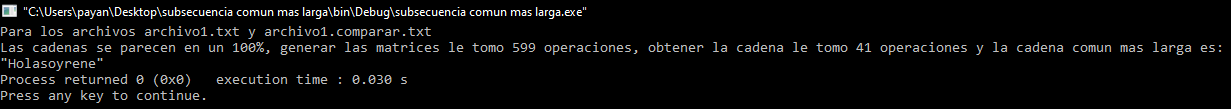
\includegraphics[width=400px,height=110px]{captura1}
		\caption{Ejecucion del programa en el primer par de archivos}
	\end{figure}
	\begin{figure}[H]
		\centering
		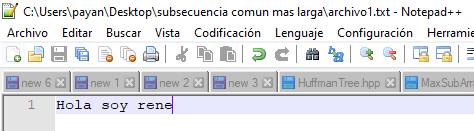
\includegraphics[width=400px,height=110px]{captura2}
		\caption{Primer archivo}
	\end{figure}
	\begin{figure}[H]
		\centering
		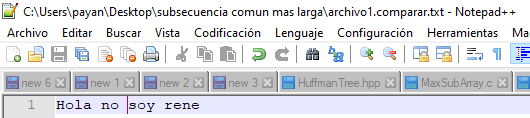
\includegraphics[width=400px,height=110px]{captura3}
		\caption{Primer archivo de comparacion}
	\end{figure}
	Como se puede apreciar, la subsecuencia comun mas larga es "Hola soy rene", ya que esta presente en ambos, por lo que el archivo de comparacion es 100$\%$ parecido al archivo original y podriamos decir que es un plagio acorde al algoritmo, pero en realidad la intencion entre ambos es completamente lo opuesto. Es decir el algoritmo esta correcto, pero en la realidad los archivos no son un plagio en si, de hecho expresan lo opuesto.\\
	Ahora se continuan las comparaciones de los 4 archivos de texto faltantes, estos a diferencia del primero seran generados aleatoriamente.\\
	\begin{figure}[H]
		\centering
		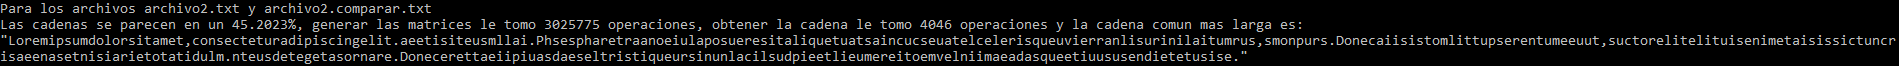
\includegraphics[width=400px,height=50px]{captura4}
		\caption{Ejecucion del programa en el segundo par de archivos}
	\end{figure}
	\begin{figure}[H]
		\centering
		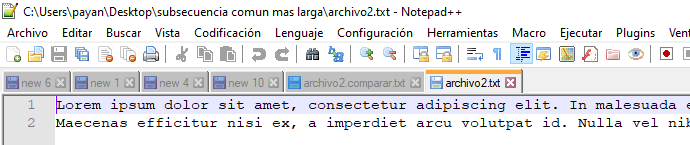
\includegraphics[width=400px,height=110px]{captura5}
		\caption{Segundo archivo}
	\end{figure}
	\begin{figure}[H]
		\centering
		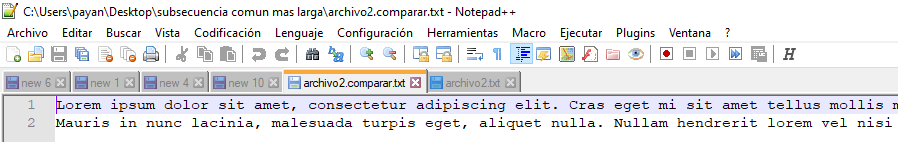
\includegraphics[width=400px,height=110px]{captura6}
		\caption{Segundo archivo de comparacion}
	\end{figure}
	\begin{figure}[H]
		\centering
		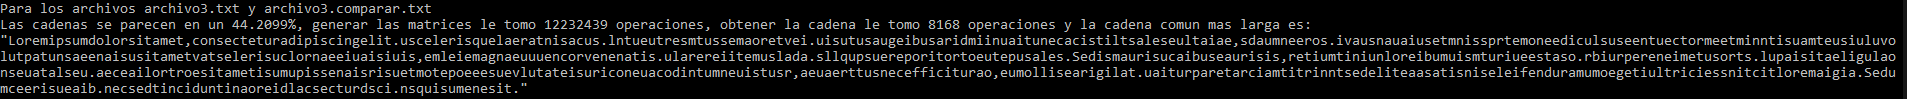
\includegraphics[width=400px,height=50px]{captura7}
		\caption{Ejecucion del programa en el tercer par de archivos}
	\end{figure}
	\begin{figure}[H]
		\centering
		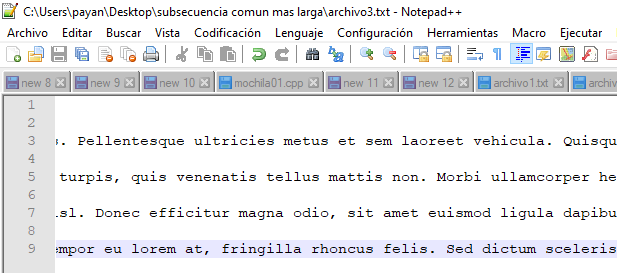
\includegraphics[width=400px,height=110px]{captura8}
		\caption{Tercer archivo}
	\end{figure}
	\begin{figure}[H]
		\centering
		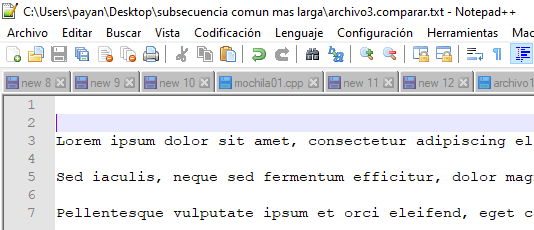
\includegraphics[width=400px,height=110px]{captura9}
		\caption{Tercer archivo de comparacion}
	\end{figure}
		\begin{figure}[H]
		\centering
		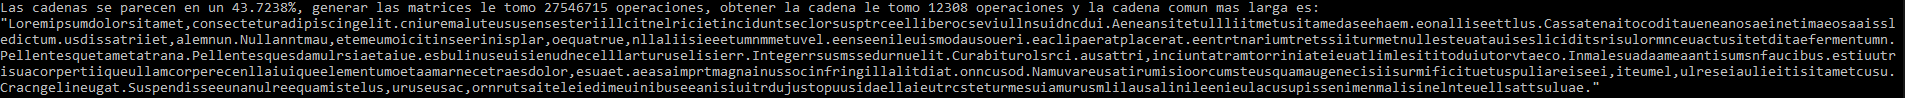
\includegraphics[width=400px,height=50px]{captura10}
		\caption{Ejecucion del programa en el cuarto par de archivos}
	\end{figure}
	\begin{figure}[H]
		\centering
		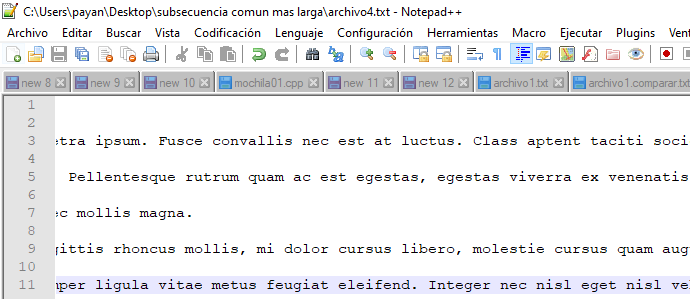
\includegraphics[width=400px,height=110px]{captura11}
		\caption{Cuarto archivo}
	\end{figure}
	\begin{figure}[H]
		\centering
		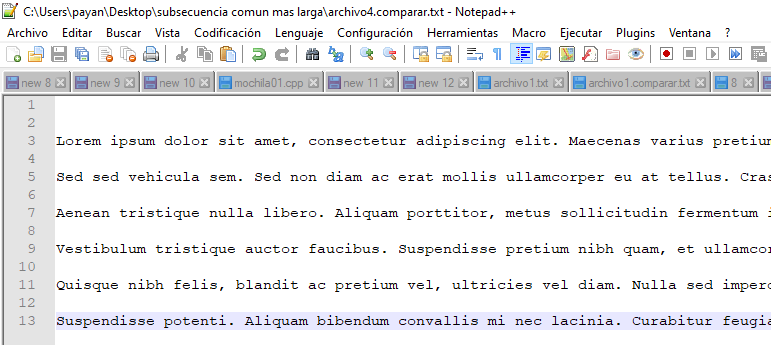
\includegraphics[width=400px,height=110px]{captura12}
		\caption{Cuarto archivo de comparacion}
	\end{figure}
		\begin{figure}[H]
		\centering
		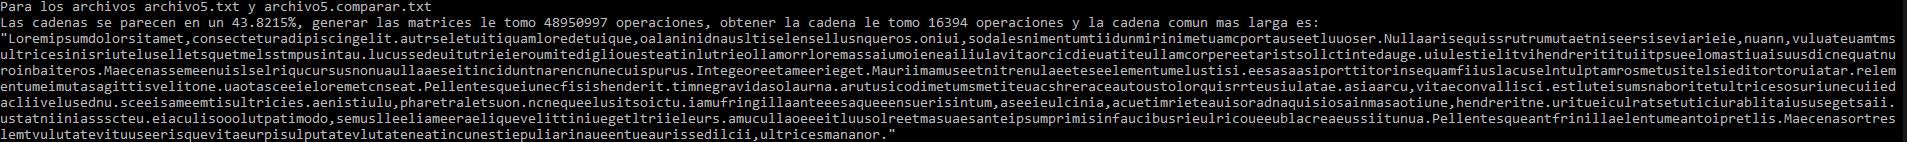
\includegraphics[width=400px,height=75px]{captura13}
		\caption{Ejecucion del programa en el quinto par de archivos}
	\end{figure}
	\begin{figure}[H]
		\centering
		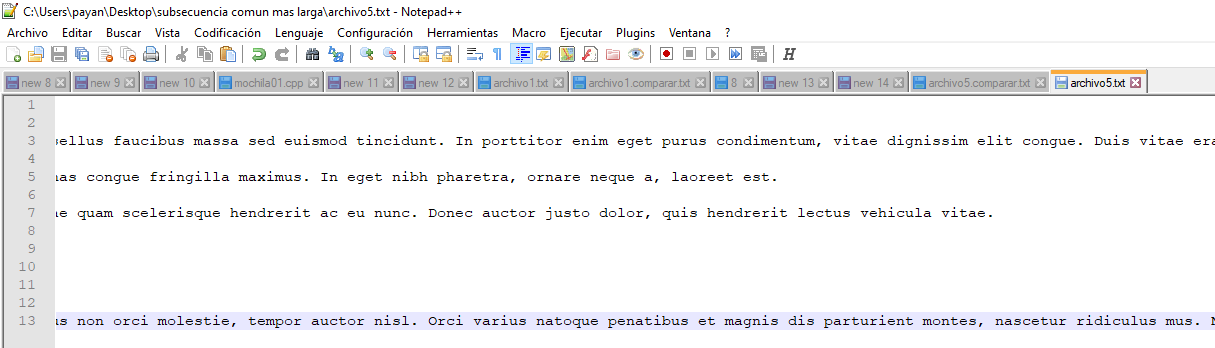
\includegraphics[width=400px,height=110px]{captura14}
		\caption{Quinto archivo}
	\end{figure}
	\begin{figure}[H]
		\centering
		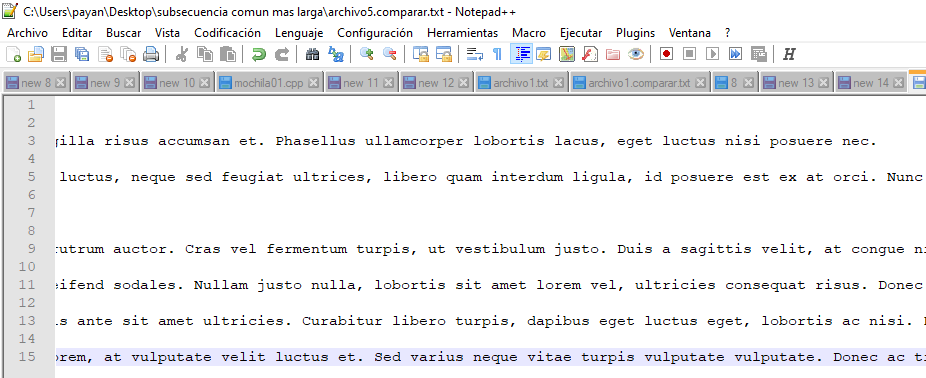
\includegraphics[width=400px,height=110px]{captura15}
		\caption{Quinto archivo de comparacion}
	\end{figure}
	Cabe mencionar que aunque este algoritmo es relativamente rapido y muy efectivo para encontrar las subsecuencias tambien consume mucha memoria RAM, ya que requiere de 2 matrices, una de enteros y otra de caracteres del tamaño nxm donde n es el numero de caracteres del archivo 1 y m el del archivo 2, lo que significa que puede llegar a consumir una gran cantidad de memoria en archivos muy grandes.\\
	\begin{figure}[H]
		\centering
		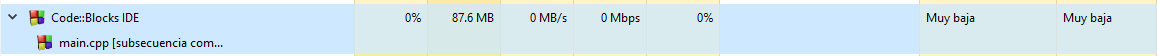
\includegraphics[width=400px,height=50px]{captura16}
		\caption{Consumo de memoria RAM durante la ejecucion del programa}
	\end{figure}
	Para probar el punto anterior, removi los free de todo el programa para poder tener un aproximado del consumo a travez de los 5 archivos.\\
	\subsection{Implementar el algoritmo de multiplicacion de matrices.} 
	Para este algoritmo se implemento un programa que recibiera el numero de matrices y sus configuraciones por consola, luego aplica el algoritmo de multiplicacion de matrices y por ultimo imprime la configuracion de parentecis mas optima y la cantidad de operaciones de la misma, asi como las matrices con las que se llego a esa conclusion (m y s) e informacion del tiempo computacional.\\
	\begin{figure}[H]
		\centering
		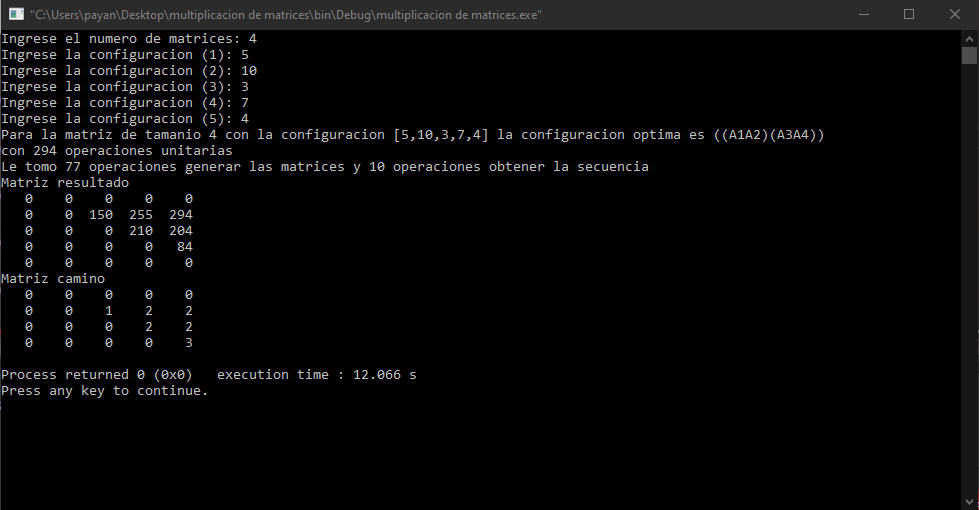
\includegraphics[width=400px,height=200px]{captura17}
		\caption{Ejecucion del programa en el primer ejemplo (tomado del video de la clase)}
	\end{figure}
	Como se puede apreciar en este ejemplo (n = 4, p = [5,10,3,7,4]) el algoritmo menciona que la parentizacion mas optima es $(A_1*A_2)(A_3*A_4)$ con un total de 294 operaciones unitarias. Para esta configuracion particular de matrices se tienen las siguientes combinaciones:
	\begin{itemize}
		\item $((A_1(A_2*A_3))A_4)$ con 700 productos escalares:
		\begin{itemize}
			\item $A_2*A_3$ = 10*3*7 = 210 operaciones con una matriz resultado de 10x7
			\item $A_1(A_2*A_3)$ = 5*10*7 = 350 operaciones con una matriz resultado de 5x7
			\item $((A_1(A_2*A_3))A_4)$ = 5*7*4 = 140 operaciones con una matriz resultado de 5x4
		\end{itemize}
		\item $A_1((A_2*A_3)A_4)$ con 690 productos escalares:
		\begin{itemize}
			\item $A_2*A_3$ = 10*3*7 = 210 operaciones con una matriz resultado de 10x7
			\item $(A_2*A_3)A_4$ = 10*7*4 = 280 operaciones con una matriz resultado de 10x4
			\item $A_1((A_2*A_3)A_4)$ = 5*10*4 = 200 operaciones con una matriz resultado de 5x4
		\end{itemize}
		\item $A_1(A_2(A_3*A_4))$ con 404 productos escalares:
		\begin{itemize}
			\item $A_3*A_4$ = 3*7*4 = 84 operaciones con una matriz resultado de 3x4
			\item $A_2(A_3*A_4)$ = 10*3*4 = 120 operaciones con una matriz resultado de 10x4
			\item $A_1(A_2(A_3*A_4))$ = 5*10*4 = 200 operaciones con una matriz resultado de 5x4
		\end{itemize}	
		\item $(((A_1*A_2)A_3)A_4)$ con 395 productos escalares:
		\begin{itemize}
			\item $A_1*A_2$ = 5*10*3 = 150 operaciones con una matriz resultado de 5x3
			\item $(A_1*A_2)A_3$ = 5*3*7 = 105 operaciones con una matriz resultado de 5x7
			\item $(((A_1*A_2)A_3)A_4)$ = 5*7*4 = 140 operaciones con una matriz resultado de 5x4
		\end{itemize}	
		\item $(A_1*A_2)(A_3*A_4)$ con 294 productos escalares:
		\begin{itemize}
			\item $A_1*A_2$ = 5*10*3 = 150 operaciones con una matriz resultado de 5x3
			\item $A_3*A_4$ = 3*7*4 = 84 operaciones con una matriz resultado de 3x4
			\item $(A_1*A_2)(A_3*A_4)$ = 5*3*4 = 60 operaciones con una matriz resultado de 5x4
		\end{itemize}
	\end{itemize}
	\begin{figure}[H]
		\centering
		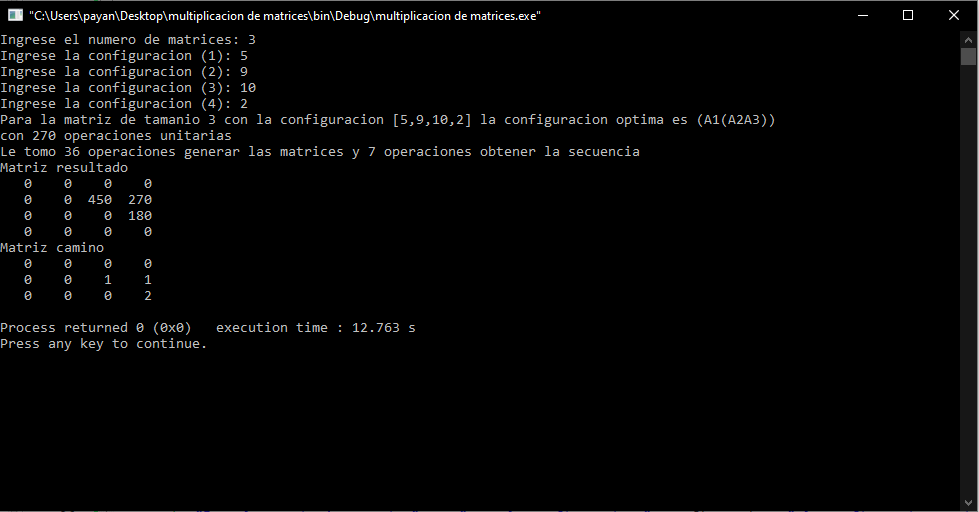
\includegraphics[width=400px,height=200px]{captura18}
		\caption{Ejecucion del programa en el segundo ejemplo}
	\end{figure}
	Como se puede apreciar en este ejemplo (n = 3, p = [5,9,10,2]) el algoritmo menciona que la parentizacion mas optima es $(A_1(A_2*A_3))$ con un total de 270 operaciones unitarias. Para esta configuracion particular de matrices se tienen las siguientes combinaciones:
	\begin{itemize}
		\item $((A_1*A_2)*A_3)$ con 550 productos escalares:
		\begin{itemize}
			\item $A_1*A_2$ = 5*9*10 = 450 operaciones con una matriz resultado de 5x10
			\item $((A_1*A_2)*A_3)$ = 5*10*2 = 100 operaciones con una matriz resultado de 5x2
		\end{itemize}	
		\item $(A_1(A_2*A_3))$ con 270 productos escalares:
		\begin{itemize}
			\item $A_2*A_3$ = 9*10*2 = 180 operaciones con una matriz resultado de 9x2
			\item $A_1(A_2*A_3)$ = 5*9*2 = 90 operaciones con una matriz resultado de 5x2
		\end{itemize}		
	\end{itemize}
	\section{Conclusiones}	
	\subsection{Payán Téllez René}
	Puedo concluir que los 2 algoritmos de programacion dinamica que se usaron durante esta practica, fueron mas dificiles de entender al menos para mi, que implementar como tal, considero que esto cumple con un algoritmo de programacion dinamica de ser una solucion rapida que a su vez se programe de forma rapida y de una solucion aunque no la mas optima a un problema extremadamente complicado, de ahi que entender el como funciona el algoritmo y porque funciona es mas complejo que programarlo como tal. Del primer algoritmo (LCS) encontre varios usos fascinantes en la vida real que van desde lo mas sencillo como un buscador o comparador de texto hasta lo mas complejo como analisis de cadenas de ADN o como herramienta en bio-informatica, lo cual me sorprendio de que un algoritmo tan directo pueda tener usos tan avanzados, tambien debo aclarar que el algoritmo, como mencione antes no es muy eficiente en el aspecto de memoria, ya que puede consumir una enorme cantidad de la misma en pequeños archivos, es decir que para comparar documentos mas grandes podria vaciar la memoria. Del segundo algoritmo, es quiza el que mas se me dificulto para entenderlo, pero una vez que lo hice, cabe aclarar que es extremadamente poderoso y tiene un enorme alcance para optimzar operaciones matematicas, de los usos que se me ocurren es en la criptografia donde normalmente se multiplican varias matrices, este algoritmo permitiria hacerlo muy rapido.\\
	\includegraphics[height=120px,width=120px]{Rene}
	\section{Anexo}			
	\section{Bibliografia}
	{[}1{]}\url{http://www.lcc.uma.es/~av/Libro/CAP3.pdf}\\
	{[}2{]}\url{https://medium.com/@joseguillermo_/qu\%C3\%A9-es-la-complejidad-algor\%C3\%ADtmica-y-con-qu\%C3\%A9-se-come-2638e7fd9e8c}\\
	{[}3{]}\url{http://cms.dm.uba.ar/materias/1ercuat2009/optimizacion/Maurette_Ojea.pdf}\\
	{[}4{]}\url{https://www.geeksforgeeks.org/longest-common-subsequence-dp-4/}\\
	{[}5{]}\url{https://sodocumentation.net/es/dynamic-programming/topic/7996/matriz-de-multiplicacion-de-la-cadena}\\
\end{document}